\chapter{Representations of Logical Functions}
\graphicspath{ {./chapter02/FigWork} }

\section{Helpfull Stuff}

\begin{tabular}{lll}
    \begin{tabular}{c|c||c}
        A & B & A*B \\ \hline \hline
        0 & 0 & 0   \\ \hline
        0 & 1 & 0   \\ \hline
        1 & 0 & 0   \\ \hline
        1 & 1 & 1   \\
    \end{tabular}
    &
    \begin{tabular}{c|c||c}
        A & B & A+B \\ \hline \hline
        0 & 0 & 0   \\ \hline
        0 & 1 & 1   \\ \hline
        1 & 0 & 1   \\ \hline
        1 & 1 & 1   \\
    \end{tabular}
    &
    \begin{tabular}{c||c}
        A & A' \\ \hline \hline
        0 & 1   \\ \hline
        1 & 0   \\
    \end{tabular} \\
\end{tabular}
\vspace{0.2in}


\includegraphics{../Fig/forms}
\vspace{0.2in}

\begin{tabular}[ht]{l|l|l}
    & Regular Algebra        & Boolean Algebra \\ \hline \hline
    Performed First    & Parenthesis        & Parenthesis \\ \hline
    & Exponents            & Not  \\  \hline
    & multiplication/division & And \\  \hline
    Performed Last    & addition/subtraction     & Or \\
\end{tabular}

\vspace{0.2in}

\begin{tabular}[ht]{|c|c|c|}\hline
    Axiom    &    Primary &    Dual    \\ \hline
    1.    &    x+0=x    &    x*1=x    \\ \hline
    2.    &    x+1=1    &    x*0=0    \\ \hline
    3.    &    x+x=x    &    x*x=x    \\ \hline
    4.    &    x''=x    &             \\ \hline
    5.    &    x+x'=1    &    x*x'=0    \\ \hline
    6.    &    x+y=y+x    &    x*y=y*x\\ \hline
    7.    & x+(y+z)=(x+y)+z&x*(y*z)=(x*y)*z \\ \hline
    8.    & x*(y+z)=x*y+x*z  & x+(y*z)=(x+y)*(x+z)  \\ \hline
    9.    & (x+y)'=x'*y'  & (x*y)'=x'+y' \\ \hline
\end{tabular}

%%%%%%%%%%%%%%%%%%%%%%%%%%%%%%%%%%%%%%%%%%%%%%%%%%%%
%% Here are terms that the students define
%%%%%%%%%%%%%%%%%%%%%%%%%%%%%%%%%%%%%%%%%%%%%%%%%%%%
\section{Definitions}
Define each of the following. Some of the definitions should use terms you've defined.
\begin{description}
    \item[Minterm]
    \item[Maxterm]
    \item[Minterm Trick]
    \item[Expansion Trick]
\end{description}

%%%%%%%%%%%%%%%%%%%%%%%%%%%%%%%%%%%%%%%%%%%%%%%%%%%%
%% Here are the problems
%%%%%%%%%%%%%%%%%%%%%%%%%%%%%%%%%%%%%%%%%%%%%%%%%%%%
\section{Problems}
Solve the following problems in the space provided.

\begin{enumerate}
    \item Given the circuit diagram below, produce the corresponding truth table.

        \begin{tabular}{ll}
            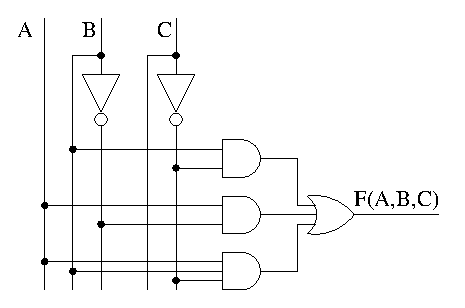
\includegraphics{../Fig/cd-tt}
            &
            \begin{tabular}{c|c|c||c}
                A & B & C & F(A,B,C) \\ \hline \hline
                0 & 0 & 0 &   \\ \hline
                0 & 0 & 1 &   \\ \hline
                0 & 1 & 0 &   \\ \hline
                0 & 1 & 1 &   \\ \hline
                1 & 0 & 0 &   \\ \hline
                1 & 0 & 1 &   \\ \hline
                1 & 1 & 0 &   \\ \hline
                1 & 1 & 1 &   \\
            \end{tabular}
        \end{tabular}

        \begin{onlysolution}
            This problem has not been solved yet.  Please go into the work2.tex \LaTeX file and create the solution.
        \end{onlysolution}

        %% \item[Determine the symbolic for the circuit.]
        %% \includegraphics{./FigWork/cd-sym-easy}

        %% \item[Determine the symbolic for the circuit.]
        %% \includegraphics{./FigWork/cd-sym-hard}

    \item Given the symbolic expression below, produce the corresponding circuit diagram.

        \begin{tabular}{lp{2in}}
            F(A,B,C)=AB'+A(B'+C)  & \\
        \end{tabular}
        \begin{onlysolution}
            This problem has not been solved yet.  Please go into the work2.tex \LaTeX file and create the solution.
        \end{onlysolution}
        \vspace{3cm}

    \item Given the symbolic expression below, produce the corresponding circuit diagram.

        \begin{tabular}{lp{2in}}
            F(A,B,C,D)=A(BC+A(C'+D)')' + B'CD'  & \\
        \end{tabular}
        \begin{onlysolution}
            This problem has not been solved yet.  Please go into the work2.tex \LaTeX file and create the solution.
        \end{onlysolution}
        \vspace{3cm}

    \item Given the symbolic expression below, produce the corresponding truth table.

        F(A,B,C) = AB'+A(B'+C)

        \begin{tabular}{c|c|c|c|c||c}
            A & B & C &   &    &  F(A,B,C) \\ \hline \hline
            0 & 0 & 0 &   &    &    \\ \hline
            0 & 0 & 1 &   &    &    \\ \hline
            0 & 1 & 0 &   &    &    \\ \hline
            0 & 1 & 1 &   &    &    \\ \hline
            1 & 0 & 0 &   &    &    \\ \hline
            1 & 0 & 1 &   &    &    \\ \hline
            1 & 1 & 0 &   &    &    \\ \hline
            1 & 1 & 1 &   &    &    \\
        \end{tabular}

    \item Given the symbolic expression below, produce the corresponding truth table.

        F(A,B,C,D)=A(BC+A(C'+D)')' + B'CD'

        \begin{tabular}{c|c|c|c||p{0.1in}|p{0.2in}|p{0.2in}|p{0.2in}|p{0.2in}||c}
            A & B & C & D &   &    &  &  &  & F(A,B,C,D) \\ \hline \hline
            0 & 0 & 0 & 0 &   &    &  &  &  &   \\ \hline
            0 & 0 & 0 & 1 &   &    &  &  &  &   \\ \hline
            0 & 0 & 1 & 0 &   &    &  &  &  &   \\ \hline
            0 & 0 & 1 & 1 &   &    &  &  &  &   \\ \hline
            0 & 1 & 0 & 0 &   &    &  &  &  &   \\ \hline
            0 & 1 & 0 & 1 &   &    &  &  &  &   \\ \hline
            0 & 1 & 1 & 0 &   &    &  &  &  &   \\ \hline
            0 & 1 & 1 & 1 &   &    &  &  &  &   \\ \hline
            1 & 0 & 0 & 0 &   &    &  &  &  &   \\ \hline
            1 & 0 & 0 & 1 &   &    &  &  &  &   \\ \hline
            1 & 0 & 1 & 0 &   &    &  &  &  &   \\ \hline
            1 & 0 & 1 & 1 &   &    &  &  &  &   \\ \hline
            1 & 1 & 0 & 0 &   &    &  &  &  &   \\ \hline
            1 & 1 & 0 & 1 &   &    &  &  &  &   \\ \hline
            1 & 1 & 1 & 0 &   &    &  &  &  &   \\ \hline
            1 & 1 & 1 & 1 &   &    &  &  &  &   \\
        \end{tabular}

    \item Given the truth table below, produce the corresponding symbolic expression.

        \begin{tabular}{c|c|c||c|c|c}
            A & B & C & F(A,B,C)    & minterm & maxterm    \\ \hline
            0 & 0 & 0 & 0        &        &     \\ \hline
            0 & 0 & 1 & 1        &         &    \\ \hline
            0 & 1 & 0 & 1        &         &    \\ \hline
            0 & 1 & 1 & 1        &         &    \\ \hline
            1 & 0 & 0 & 1        &         &    \\ \hline
            1 & 0 & 1 & 0        &         &    \\ \hline
            1 & 1 & 0 & 0        &         &    \\ \hline
            1 & 1 & 1 & 1        &         &    \\
        \end{tabular}
        \vspace{1cm}

    \item Given the word state below, produce the corresponding truth table.
        Design a circuit with two 2-bit inputs called $A = a_1 a_0$ and  $B = b_1 b_0$
        The single bit output $F$ should equal 1 when A+B $>$ 6, otherwise $F$
        should equal 0.

        \begin{tabular}{c|c|c|c||c|c||c}
            $a_1$ & $a_0$ & $b_1$ & $b_0$ & A  & B & $F(a_1, a_0, b_1, b_0)$     \\ \hline
            0 & 0 & 0 & 0 &  &  &   \\ \hline
            0 & 0 & 0 & 1 &  &  &   \\ \hline
            0 & 0 & 1 & 0 &  &  &   \\ \hline
            0 & 0 & 1 & 1 &  &  &   \\ \hline
            0 & 1 & 0 & 0 &  &  &   \\ \hline
            0 & 1 & 0 & 1 &  &  &   \\ \hline
            0 & 1 & 1 & 0 &  &  &   \\ \hline
            0 & 1 & 1 & 1 &  &  &   \\ \hline
            1 & 0 & 0 & 0 &  &  &   \\ \hline
            1 & 0 & 0 & 1 &  &  &   \\ \hline
            1 & 0 & 1 & 0 &  &  &   \\ \hline
            1 & 0 & 1 & 1 &  &  &   \\ \hline
            1 & 1 & 0 & 0 &  &  &   \\ \hline
            1 & 1 & 0 & 1 &  &  &   \\ \hline
            1 & 1 & 1 & 0 &  &  &   \\ \hline
            1 & 1 & 1 & 1 &  &  &   \\
        \end{tabular}

        %% \index[Complete the timing diagram for the function $F(A,B,C) = A'B + AB'C$.]
        %% 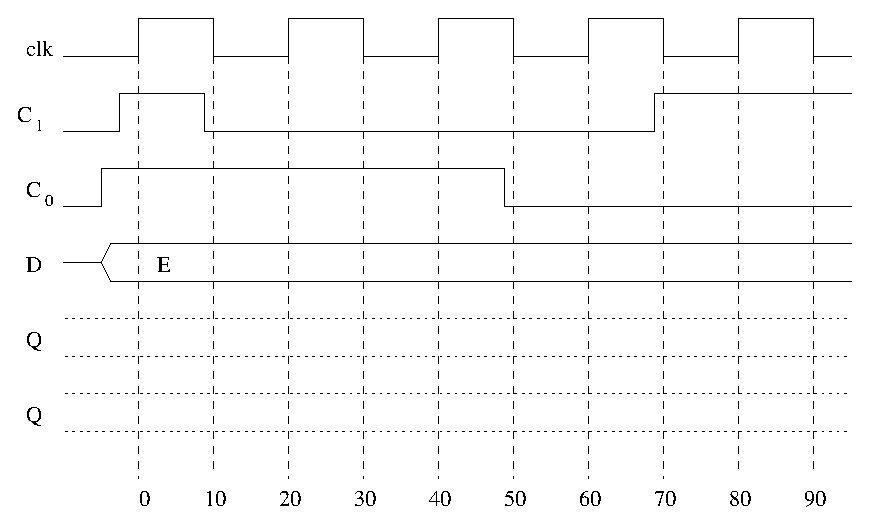
\includegraphics{./FigWork/time}
\end{enumerate}
